% (c) Jakub Stejskal
% Master Thesis
% Performance Testing and Analysis of Qpid-Dispatch Router
% Chapter 3

\chapter{Messaging Performance Tool}
\label{Messaging Performance Tool}
% https://github.com/orpiske/msg-perf-tool
The performance of \emph{Message-Oriented Middleware} (MOM) \cite{CURRY:MOM} is one of the most critical elements of quality assurance for enterprise integration systems. There are multiple messaging components developed in the Red Hat company such as messaging clients, Message Broker, Message Router (Qpid-dispatch service) or stream-like message distributions tools---Kafka. All of these software needs performance testing to ensure quality standards of MOM. Note that we will shorten the term the messaging client to just client in this thesis.

The~Message Broker is an example of MOM. Its main purpose is to receive, store and distribute messages, which are sent and received by clients. Users choose MOM for message distribution to reduce the development time and cost of their own solution. Another benefit of using specialized MOM is robustness and guaranteed performance. The performance capabilities of a MOM are critical attributes to its users, because being able to handle a large amount of transactions in a timely manner is a key characteristic of MOM. Good example are automated systems, where components communicates with each other by command exchange. The amount of exchanged commands is heavily dependent on the system size and since we want to get the results as soon as possible we need to ensure smooth and quick message exchange.

\emph{Maestro} (or Messaging Performance Tool) \cite{ORPISKE:MSGPT} is a testing system designed for testing the performance of MOM. The Maestro is deployed as a cluster system on several machines. A~typical deployment consist of one node for Maestro Broker, one or more for Maestro Senders, and one or more for Maestro Receivers and the SUT. The architecture of Maestro system, depicted in the Figure \ref{fig:msg_perf_tool}, consists of the following components:

\begin{description}
	\setlength\itemsep{0em}
	\item \textbf{Maestro Broker}\,---\,can be any \emph{Message Queuing Telemetry Transport\footnote{MQTT\,---\,\url{http://mqtt.org/}} (MQTT)} capable broker with several topics. The topic is a queue with a name where other messaging services can listen on the traffic. This component takes care of distribution of control messages between other cluster components such as Maestro Clients and MPT Backend.
	\item \textbf{Meastro Clients}\,---\,this component contains the client API as well as the test scripts for each test case. Moreover it contains a~sub-component called Reporter which interprets the test data to user in form of web data visualizations.
	\item \textbf{MPT Back-end}\,---\,consists of sender, receiver and inspector parts. Sender and receiver handle message sending to the SUT and receiving from SUT. Inspector monitors workload over the SUT and reports collected performance metrics to the data server. Maestro currently has two backends:
	\begin{itemize}
		\item \textbf{Java}\,---\,used for JMS-based\footnote{JMS\,---\,Java Message Service} testing, including \emph{Advanced Message Queuing Protocol (AMQP)} \cite{OASIS:AMQP}, OpenWire and Core protocols.
		\item \textbf{C}\,---\,used for AMQP and \emph{Streaming Text Oriented Messaging Protocol\footnote{STOMP\,---\,\url{https://stomp.github.io/}} (STOMP)} protocol testing.
	\end{itemize}
\end{description}

\begin{figure}[H]
  \centering
  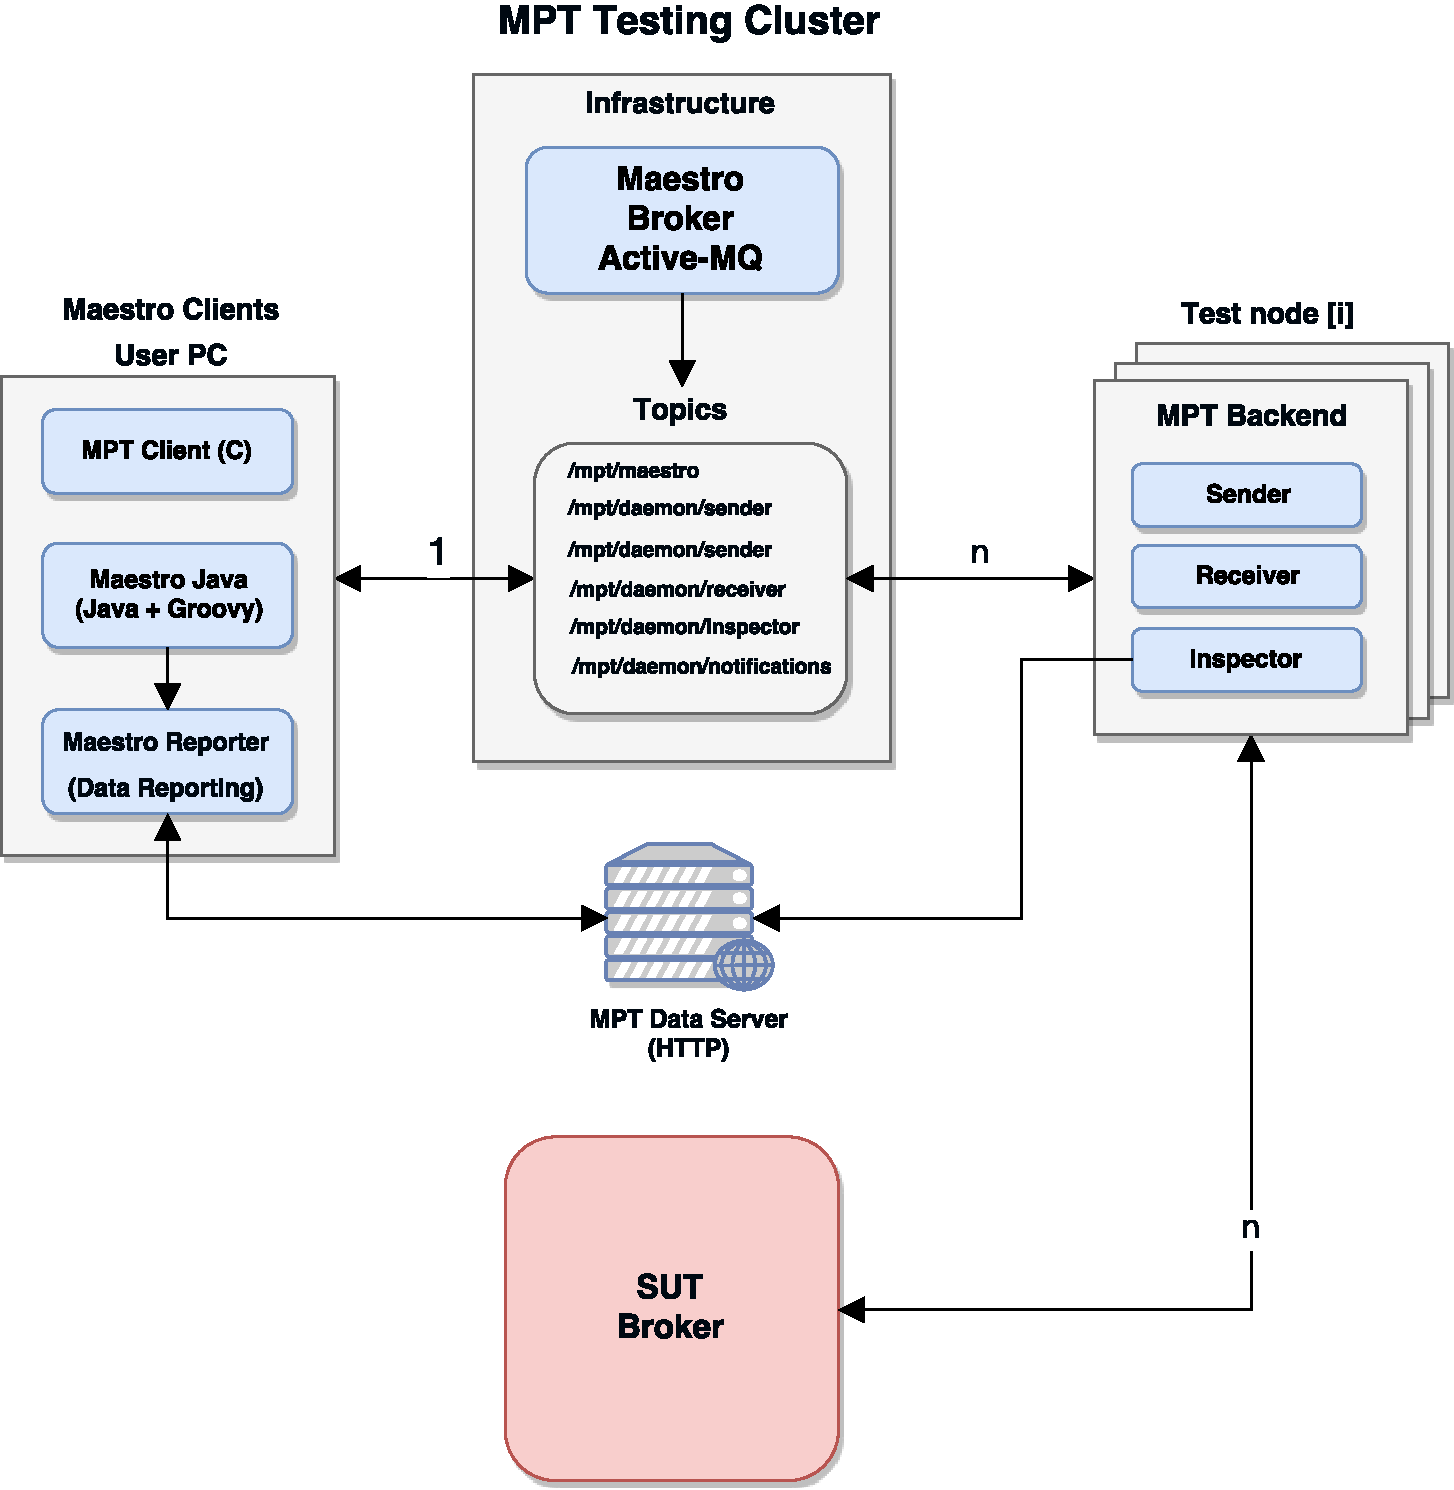
\includegraphics[width=15cm]{obrazky-figures/msg_perf_tool.pdf}
  \caption{The architecture of the Maestro. The Maestro contains Maestro Clients as a front-end; Maestro Broker as a message distributor; and sender, receiver and inspectors as a backend.}
  \label{fig:msg_perf_tool}
\end{figure}

\newpage

\section{Test Case Scenario}
The test is basically a generation of huge amount of messages followed by sending them to SUT and then receiving them. The configuration of each test case is specified by several options defined in the Groovy\footnote{Groovy\,---\,object-oriented programming language for Java platform \url{http://groovy-lang.org/}} script which influences the test behavior with the following elements:

\begin{itemize}
	\setlength\itemsep{0em}
	\item \textbf{message size}\,---\,size of the generated test message in bytes,
	\item \textbf{number of connected clients}\,---\,the count of senders and receivers connected to the SUT,
	\item \textbf{test duration (time or load)}\,---\,the end condition of each test; can be specified by time, limit or message count,
	\item \textbf{message rate}\,---\,the desired rate that the system should try to maintain through the test (0 for unbounded rate).
\end{itemize}

The test script is also responsible for starting and stopping the test. Moreover the test case can be extended by the so called test profile. The script will then also be responsible for increasing or decreasing the workload on the SUT during the test scenario. This load can be modified by increasing either the target rate or the number of parallel connections. With multiple combinations of these options we can create a lot of test cases with different loads for the SUT and thus achieve a broad coverage of testing. Every test produces its own logs which are processed by the reporting sub-component on the client side and used for monitoring the metrics. Maestro Reporter produces data visualizations, such as the test overview and charts (rate based on time and latency over the test) from these logs.

\section{Communication Between Components}
\label{Communication Between Components}
The actual communication between components during the test cases is realized using the Maestro Protocol\,---\,a binary protocol implemented on top of the MessagePack\footnotemark{}. For the message exchange between nodes it currently uses MQTT protocol (version 3.1.1) and for sending the testing data to the data server it uses HTTP protocol (version 1.1). The messages exchanged between the peers of testing cluster are called notes.

\footnotetext{Messagepack\,---\,\url{https://msgpack.org/}}

Each note has a specific format consisting of three parts. First is the \emph{Type} which is short integer that identifies the purpose of the note, and is one of the following values:

\begin{itemize}
	\setlength\itemsep{0em}
	\item \textbf{Request (0)}\,---\,a note sent by a controller node to the test peers,
	\item \textbf{Response (1)}\,---\,a note sent by a testing peer as a response for a request,
	\item \textbf{Notification (2)}\,---\,a note sent by a testing peer as a reaction to an event.
\end{itemize}
The second part is the \emph{Command} which identifies the action to be executed or, in some cases, that was executed. Currently, there are 18 commands represented by a long integer. And the last part is the \emph{Payload} which refers to the data carried by the note as part of its command. Detailed description of commands and its payload is available in Appendix \ref{AP:commands}.


\section{Measuring Process}
\label{Measuring Process}
After the dynamic test generation, with options from the test file, the measuring process starts. Senders will start sending messages to the SUT, while Inspector starts monitoring the behavior of the SUT and sends measured data to the data server. For monitoring purpose, Inspector uses the Broker management interface\,---\,a REST interface that exposes (via HTTP protocol) an internal JVM\footnote{JVM\,---\,Java Virtual Machine} and Broker detailed information. The actual data collection by Inspector is straightforward:

\begin{enumerate}
	\setlength\itemsep{0em}
	\item Inspector sends a HTTP request with the \emph{JavaScript Object Notation\footnotemark{} (JSON)} content to the Broker REST interface.
	\item Broker evaluates the request and sends response to the Inspector.
	\item Inspector collects the response.
\end{enumerate}
Note that errors occurred during the collection may cause the test case to fail.

\footnotetext{JSON\,---\,\url{https://www.json.org/}}

However, there are two problem factors; the first is that the Inspector should not influence the performance of the SUT. Current solution for the information collection works like the management interface method call with request for information and response retrieval. During this call, the method usually involves locks to guarantee the thread safety and exclusive access. However, calling this method too often can cause a significant Broker performance degradation. In order to reduce this risk, the inspector enforces a collection interval of 10 seconds and restricts usage only to selected operations. This strategy reduces the hits on management interface to 2 or 3 hits every 10 seconds and presents a suitable performance.

The other problem factor is the large size of the stored logs. This is mitigated by the usage of the compression methods. However, compressed logs can still fill the whole hard drive during the long test-run and so old logs has to be erased at some point of time. Collected logs can be safely erased when the test is completed. Currently the Maestro generates about 1\,Gb of uncompressed data per hour of testing.

%Inspector also monitor node with broker (CPU, memory size)?

%No. There's a new module being developed for that, which runs on top of Prometheus and monitors both the system and the test cluster: http://msg-qe-dev-01.tpb.lab.eng.brq.redhat.com:3000


\subsection{Testing Metrics}
\label{Testing Metrics}
The type of metrics collected during tests depends on the cluster component. In the Table \ref{tab:maestro_metrics} we can see the summary of the metrics, which are collected for each component.

\begin{table}[H]
\centering
\caption{The summary of Maestro metrics summary collected during test cases.}
\begin{tabular}{|p{2.5cm}|p{3.5cm}|p{7cm}|}
\hline
\rowcolor[HTML]{C5E3DF}
\multicolumn{1}{|c|}{\textbf{Component}} & \multicolumn{1}{c|}{\textbf{Metrics}} & \multicolumn{1}{c|}{\textbf{Description}}                       \\ \hline
\textbf{Sender}                          & Throughput                            & Throughput of the sender                                        \\ \hline
\textbf{Receiver}                        & Throughput                            & Throughput of the receiver                                      \\ \hline
\textbf{}                                & Latency                               & Time between send and receive messages                           \\ \hline
\textbf{Broker}			                & JVM heap memory                       & Maximum, minimum, and current Eden, Survivor, and Tenured space\footnotemark{} \\ \hline
                                         & JVM non-heap                          & PermGen or Metaspace                                            \\ \hline
                                         & Broker internals                      & Queue size and expiration count                                 \\ \hline
                                         & OS basic memory                       & Physical and swap memory usage                                  \\ \hline
                                         & OS resources                          & Count of file descriptors                                       \\ \hline
\end{tabular}
\label{tab:maestro_metrics}
\end{table}

\footnotetext{Eden, Survivor and Tenured space are internal Java memory spaces.}

Throughput of the sender or receiver refers to the message count sent/received during the performance test run. This metric is collected by each sender and receiver. On the other hand latency is collected only by receiver. This refers to the time between sending and receiving of the message and can be influenced by the Quality of Service or other parameters. Since Messaging Broker is written in Java, JVM memory metric is relevant. High JVM memory usage can point to the memory leak or bad algorithm implementation. Broker queue has size threshold and message expiration time. When no one picks-up the message from the queue after some period of time there is no need to keep old messages and its unnecessary to fill too much of the memory.

Last metric is the OS resource spending during the performance testing. It is not relevant for broker performance, but it is helpful to know e.g. the CPU usage, memory usage, etc., in case of Broker crash debugging.

\section{Collected Data Format}
\label{Collected Data Format}
Data are collected by Inspector. Inspector continuously monitors the broker and collects information about the workload. Output of this measurement should be one file for each active inspector. The broker inspector file is composed of the following columns:

\begin{itemize}
	\setlength\itemsep{0em}
	\item \textbf{Timestamp}\,---\,the date and time of the data sample in the format YYYY-MM-DD hh:mm:ss using the W3C defined standard for datetime.
	\item \textbf{Load}\,---\,size of the system load.
	\item \textbf{Open file descriptors}\,---\,number of opened filed descriptors.
	\item \textbf{Free file descriptors}\,---\,number of free file descriptors.
	\item \textbf{Free memory}\,---\,free physical memory.
	\item \textbf{Free swap memory}\,---\,swap free memory.
	\item \textbf{Swap committed}\,---\,swap committed memory.
	\item \textbf{Eden initial}\,---\,Eden initial memory.
	\item \textbf{Eden committed}\,---\,Eden committed memory.
	\item \textbf{Eden max}\,---\,Eden maximum (limit) memory.
	\item \textbf{Eden used}\,---\,Eden used memory.
	\item \textbf{Survivor initial}\,---\,Survivor initial memory.
	\item \textbf{Survivor committed}\,---\,Survivor committed memory
	\item \textbf{Survivor max}\,---\,Survivor maximum (limit) memory.
	\item \textbf{Survivor used}\,---\,Survivor used memory.
	\item \textbf{Tenured initial}\,---\,Tenured initial memory.
	\item \textbf{Tenured committed}\,---\,Tenured committed memory.
	\item \textbf{Tenured max}\,---\,Tenured max memory.
	\item \textbf{Tenured used}\,---\,Tenured used memory.
	\item \textbf{PM initial}\,---\,Permgen or Metaspace initial memory (either Permgen or Metaspace depending the JVM version).
	\item \textbf{PM committed}\,---\,Permgen or Metaspace committed memory (either Permgen or Metaspace depending the JVM version).
	\item \textbf{PM max}\,---\,Permgen or Metaspace maximum memory (either Permgen or Metaspace depending the JVM version).
	\item \textbf{PM used}\,---\,Permgen or Metaspace used memory (either Permgen or Metaspace depending the JVM version).
	\item \textbf{Queue size}\,---\,number of messages waiting for processing in the queue.
	\item \textbf{Consumers}\,---\,number of consumers connected to the queue.
	\item \textbf{Acknowledged}\,---\,number of acknowledged messages in the queue.
	\item \textbf{Expired}\,---\,number of expired messages in the queue.
\end{itemize}

Maestro sender and receiver generate another relative performance testing data. Receiver generates latency log with the following data:

\begin{itemize}
	\setlength\itemsep{0em}
	\item \textbf{Start Time-stamp}\,---\,start time of the receiving.
	\item \textbf{End Time-stamp}\,---\,end time of the receiving.
	\item \textbf{Interval Maximum}\,---\,collected maximum latency.
	\item \textbf{Interval Compressed Histogram}\,---\,compressed histogram of measurement's latency in HDR\footnotemark{} format.
\end{itemize}

Both, sender and receiver generate rate (throughput) data files. These contain data about sent or received data by each peer. Data are stored in a compressed comma-separated values (CSV) file with the following columns:

\begin{itemize}
	\setlength\itemsep{0em}
	\item \textbf{eta}\,---\,represents the estimated time of departure/arrival of the message, relative to the start of the test.
	\item \textbf{ata}\,---\,represents the actual time of departure/arrival of the message, relative to the start of the test.
\end{itemize}

\footnotetext{HDR\,---\,\url{http://hdrhistogram.github.io/HdrHistogram/JavaDoc/org/HdrHistogram/package-summary.html}}

\section{Related Works}
\label{Related Works}
% popsat podobne "existujici" reseni (samozrejme, obcas neexistuje ;), ale verim, ze zde se neco najde). Nejlepsi je i se vuci tem "related tools" vymezit (jako napr. "The tool ... cannot be used because it does not support ...")

While Maestro is relatively new system, there are only few existing performance testing tools for MOM. Noteworthy are two tools, which were used for performance testing before the maestro development. These tools are \emph{SpecJMS} \cite{SPECJMS} and \emph{JMeter}\footnote{JMeter\,---\,\url{https://jmeter.apache.org/}}, the advantages and disadvantages are described in the following.

\subsubsection*{SpecJMS}
SpecJMS is the industry-standard benchmark for evaluating the performance of enterprise message-oriented middlevare servers based on JMS. Basically, SpecJMS runs real-world scenarios, which simulate real load over the messaging topology. SpecJMS collects data during the test and then evaluates it as a score. This score is a standardized value, which represent a performance of the tested system. Each system tested by SpecJMS can be compared with another system based on the computed score. Note, that a fair comparison between a tested systems involves run the tests on the same hardware.

The great advantage of SpecJMS is the comparison between the different tested systems only based on the performance score. However, it has a poor test case capabilities, since the test cases are pre-defined by the SpecJMS developers and designed only for JMS. Nowadays, this benchmark tool is retired and is no longer supported.

\subsubsection*{JMeter}
The Apache JMeter is an open source software designed to load test the functional behavior and measure performance. JMeter system is basically an IDE written in Java, which offers a performance testing of web applications, servers and MOM (via JMS only) by a simulation of a heavy load. JMeter testing script capabilities are better then SpecJMS has. Also the JMS restriction for MOM is not very comfortable, since Qpid-dispatch can handle more than only JMS connections such as Qpid-proton, Ruby or any connection type which is able to use the AMQP protocol. The different connection type during the test can be tested by Maestro as well. Maestro also implements interior data collection about the router itself, which is very useful during the performance bug hunt.
